%0.5 Seiten
\chapter{Sensorik und Aktorik}
Was eine autonome Paketdrohne anspruchsvoller als eine herkömmliche Drohne mit Fernbedienung macht, ist vor allem die Fähigkeit, selbstständig sich zurechtzufinden und ihre Aufgabe ohne die Hilfe von Menschen zu erledigen. Um mit der Umgebung zu interagieren braucht man sowohl Sensoren, welche zur Wahrnehmung sprich zur Messung und Kontrolle von Umgebungsvariablen dienen, als auch Aktoren, welche letztendlich die Umgebung, gesteuert durch elektrische Signale, beeinflussen können. Die Sensoren sind also die Sinne, wie zum Beispiel: fühlen, sehen oder auch riechen, welche der Drohne zur Verfügung stehen, wobei die Aktorik die Arme und Beine der Drohne sind. Um also eine Drohne zu entwickeln, welche filigrane Bewegungen durchführen kann und sich überall zurechtfinden kann braucht man dementsprechend viele Sensoren. 


%1 Seite
\section{Sensorik}
Mit das Wichtigste bei einem automatisierten Projekt ist die Sensorik, denn das ist die Grundlage auf der das ganze System basiert. Ohne die richtig gewählte Sensorik ist das Projekt, in unserem Fall die Drohne nicht in der Lage sich zu recht zu Finden und ist quasi blind und somit unbrauchbar. Die Software kann noch so gut sein, jedoch hat auch sie keine Chance, wenn sie zum Beispiel die Drohne richtig positionieren soll, ohne die aktuelle Position zu kennen.\\

In diesem Kapitel geht es folglich um die Sensorik, welche wir explizit ausgewählt und verwendet haben und nicht um Beispielsweise das Gyroskop, welches in dem Flight Controller integriert ist, mit welchem wir aber nicht wirklich etwas zu tun hatten, da die Stabilitätsregelung bereits in dem Flight Controller vorprogrammiert war. Es wird einen Überblick geben, was für Sensoren sich in unserem Projekt befinden und warum wir uns für diese entschieden haben und was unsere Auswahl beeinflusst hat.

%1 Seite
\subsection{Positionssensorik}
Die Position eines Objektes kann man entweder relativ, also in Relation zu einem anderen Objekt angeben oder man gibt die Position absolut an, wie zum Beispiel bei einem GPS in Längen- und Breitengrad. Wir haben uns dazu entschieden eine Mischung aus beidem zu benutzen, da man so eine besonders hohe Genauigkeit erreichen kann.
\\
\\ Da die Drohne Pakete ausliefern können soll, brauchen wir dementsprechend einen Sensor welcher eine absolute Position wiedergibt. Um die absolute globale Position zu bestimmen, gibt es nur eine sinnvolle Möglichkeit, und zwar GPS, was für Global Positioning System steht und weltweit funktioniert. Da GPS Sensoren allerdings nur auf etwa 10 Meter genau sind und wir Pakete mit einer Genauigkeit von etwa +-5cm anfliegen wollen ist die Positionsbestimmung über GPS nicht ausreichend. Somit müssen wir weitere Sensoren zur Unterstützung verwenden. Zur genauen Lokalisierung des Pakets verwenden wir eine Kamera, die, wie in dem Kapitel Bilderkennung beschrieben, die genaue Position des Pakets ermittelt. Durch die Kamera lässt sich die Drohne sehr gut mittig über dem Paket platzieren, jedoch kann man sehr schwer die Höhe mit einer einzelnen Kamera bestimmen. Um die Höhe genau zu bestimmen bräuchte man entweder eine Stereokamera oder einen Abstandssensor, für welchen wir uns aus Kostengründen entschieden haben.

%1 Seite
\subsection{Ultraschallsensor}
Zur Bestimmung von Abständen gibt es mehrere Ansätze, mit unterschiedlichen Vor- und Nachteilen. Man kann den Abstand über die Signallaufzeit, Triangulation oder auch über die Phasendifferenz bestimmen. Am Häufigsten sind hierbei die Signallaufzeitsensoren, welche ein Sendeimpuls abgeben und die Zeit bis zu dem Echo messen. Diese Art der Sensoren lässt sich nochmal in drei Unterkategorien einordnen mit jeweils unterschiedlichen Signalarten. Es gibt elektromagnetische (wie zum Beispiel Radar), optische (hierzu zählt unter anderem Infrarot und Lidar) und akustische (Beispielsweise Ultraschall) Abstandssensoren, die alle ihre Vor- und Nachteile haben. Wir haben uns für einen Ultraschallsensor entschieden, da dieser in dem von uns gewünschtem Bereich (ca. 2 Meter) auf etwa 10cm genau ist und vor allem weil es ein besonders kostengünstiger Sensor ist. Ein Lidarsensor wäre auch eine gute Alternative, jedoch sind diese Sensoren noch deutlich teurer als herkömmliche Ultraschallsensoren.
\\
Den Ultraschallsensor haben wir direkt mit dem Raspi verbunden, da unser Flight Controller keinen Eingang für einen Ultraschallsensor vorgesehen hat und das somit am Raspi angeschlossen die sauberste Lösung ist.
\begin{figure}[h]
	\centering
	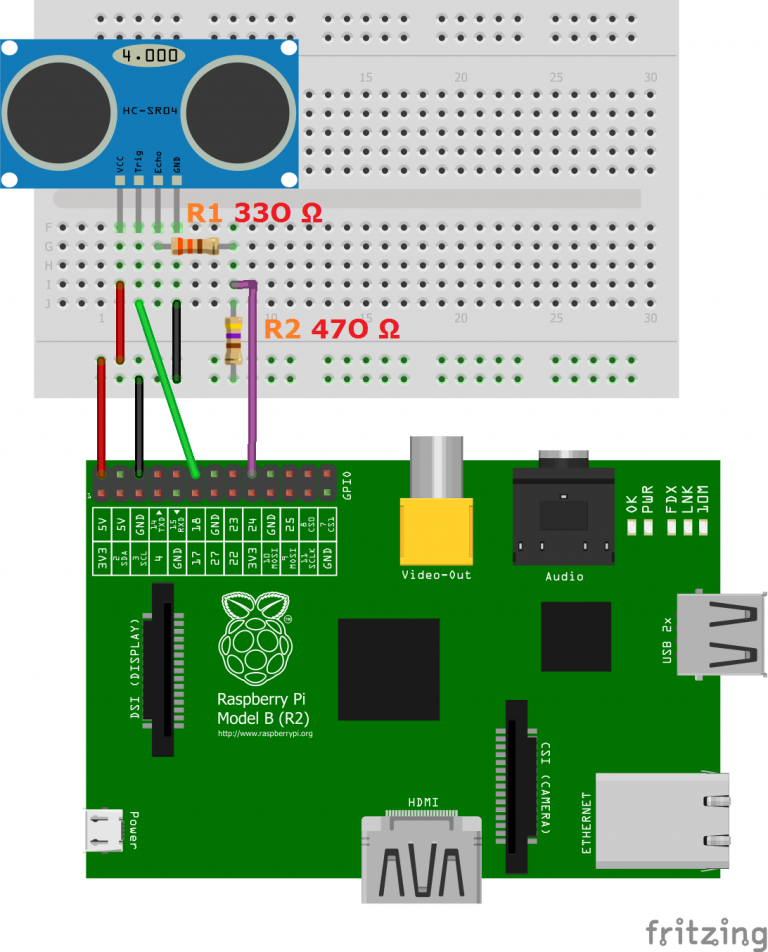
\includegraphics[scale=0.3]{"Grafiken/Ultraschallsensor.png"}
	\caption{Ultraschallsensor Schaubild\footnote{Quelle: https://tutorials-raspberrypi.de/entfernung-messen-mit-ultraschallsensor-hc-sr04/}}
	\label{fig:ultraschall}
\end{figure}
\footnotetext{Quelle: https://tutorials-raspberrypi.de/entfernung-messen-mit-ultraschallsensor-hc-sr04/}
\\
Unser Aufbau ist wie in der Abbildung \ref{fig:ultraschall} dargestellt, der Eingang des Sensors ist mit einem GPIO OUT Pin verbunden und der Ausgang über einen Spannungsteiler mit einem GPIO OUT verbunden um hier eine Spannung von 3,3V zu erreichen. Außerdem wird noch jeweils Masse mit Masse vom Raspi verbunden und 5V mit den 5V des Raspi verbunden. Es wird nun einmal die Sekunde die Entfernung nach Unten gemessen und an eine ROS Node gesendet, hierzu aber später mehr.
\\


%1.5 Seiten
\subsection{Global Positioning System (GPS)}
\subsubsection{Funktionsweise}
Wie der Name Gloabl Positioning System schon impliziert handelt es sich bei GPS um ein System, welches einem die globale Position angibt. Es gibt mehrere solcher Systeme, das jedoch weitverbreitetste ist das NAVSTAR GPS, welches von den Vereinigten Staaten von Amerika in den 1970er-Jahren entwickelt wurde und bis heute ständig renoviert und instand gehalten wird. Dieses System besteht momentan aus 31 aktiven Satelliten im Orbit, es werden jedoch nur 24 Satelliten benötigt damit die aktuelle Konstellation funktioniert. Die Überschüssigen Satelliten werden lediglich zur Verbesserung der Signalstärke und steigerung der Fehlertoleranz verwendet. Das System ist so ausgelegt, dass man an jedem Punkt auf der Erde immer Kontakt zu mindestens vier Satelliten gleichzeitig hat. Jeder Satellit sendet in einem Takt von Einer Millisekunde ein Signal, welches sowohl die Position als auch die genaue Uhrzeit des Senders, sprich des Satellitens, beinhaltet. Mit diesen Daten kann der Empfänger dann seine aktuelle Position, sprich seine Höhe sowie Längen- und Breitengrad berechnen.\\ Normalerweise sind, um einen Punkt auf der Erde zu bestimmen, nur drei Satelliten notwendig, da aber der Empfänger meist keine ausreichend präzise Uhr besitzt, welche zur Berechnung des Standorts benötigt wird, da das Signal mit Lichtgeschwindigkeit unterwegs ist und somit etwa 300 Meter pro Mikrosekunde zurücklegt, wird ein vierter Satellit zum ausgleichen des Uhrenfehlers benötigt. Aus den vier Signalen wird dann über die Signallaufzeit die aktuelle Position berechnet.
\\
\\
Jedoch hat dieses System auch seine Limitierungen, denn sobald der Empfänger keine uneingeschränkte Sicht mehr zu vier Satelliten auf einmal hat, kann er die genaue Position nicht mehr bestimmen. Das Signal von den Satelliten wird relativ schnell von Hochhäusern Brücken oder Tunneln aufgehalten, weswegen wir auch unsere Tests nicht in unserem Labor durchführen konnten, da dort keine stabile GPS Verbindung garantiert ist.

\subsubsection{Hardwareimplementierung}
Die Positionierung auf der Drohne ist bei einem GPS Empfänger sehr wichtig, da wir hier ein bestmögliches Signal haben wollen. Hierzu positionieren wir das GPS so hoch es geht, um möglichst immer eine uneingeschränkte Sicht zum Himmel zu gewährleisten.\\
Wir haben bei uns ein GPS Modul verbaut, welches sich direkt mit dem Flight Controller verbinden lässt, somit weiß dieser immer seine genaue Position und teilt sie dann dem Raspi mit.

%1.5 Seite
\subsection{Kamera}
Auch bei der Kamera hatten wir eine sehr große Auswahl von unterschiedlichen Modulen, mit den unterschiedlichsten Spezifikationen. Unsere Anforderungen waren hierbei  wie folgt:
\begin{itemize}
	\item Auflösung von mindestens 720p
	\item kompatibel mit dem Raspberry Pi
	\item Farbkamera
	\item klein und leicht
	\item preislicher Rahmen maximal 100€
	\item wenn möglich optische Bildstabilisierung
	\item wenn möglich gute Softwareunterstützung
\end{itemize}
Die größten Unterschiede, bei den mit dem Raspberry Pi kompatiblen Kameras liegen in der Größe, der Softwareunterstützung und des Interfaces. Für unseren Anwendungszweck war es von sehr großer Wichtigkeit, dass die Kamera möglichst kompakt aber vor allem leicht ist, da unsere Drohne unter den, von dem Gesetz vorgegebenen 2 kg bleiben soll und ein niedrigeres Gewicht auch eine längere Flugzeit bedeutet, welche ebenfalls sehr wichtig ist.\\
Bei dem Interface gibt es hauptsächlich zwei unterschiedliche Varianten. Variante Nummer eins ist ein normales USB-Interface, welches den Vorteil hat, dass es hier eine sehr große Auswahl gibt, jedoch sind diese Kameras meistens etwas größer und das wollen wir ja aus den oben gennanten Gründen vermeiden. Variante Nummer zwei ist die Verbindung über den SCI-Port am Raspberry Pi, das hat den Vorteil, dass man noch alle USB-Ports des Raspberry Pi frei für andere Erweiterungen hat aber auch, dass man eine deutlich bessere Kontrolle über die die Kamera hat. Man kann hier zum Beispiel die Belichtungszeit aber auch noch viele andere Parameter verstellen, was bei einer günstigen USB-Kamera meist gar nicht richtig geht oder nur sehr schwer zu realisieren ist.\\
Bei der Softwareunterstützung war uns wichtig, dass es eine sehr weit verbreitete Kamera ist, da dies meist bedeutet, dass es auch eine große Community gibt, die oft sehr hilfsbereit ist. Außerdem bedeutet das auch, dass es bereits viel Software gibt und man somit einige elementare Funktionen übernehmen kann und man somit mehr Zeit für die Projektspezifische Software hat.\\
\\
Nach einer gründlichen Recherche hatten wir eine engere Auswahl an Kameras zusammengestellt, bei der wir uns letztendlich für das Raspberry Pi Camera Module entschieden haben, da diese schon vor Ort war und wir somit direkt mit den Versuchen starten konnten. Ein weiterer Grund war die sehr gute Software Unterstützung, da die Kamera direkt für den Raspberry Pi entwickelt wurde. Außerdem hatten wir somit auch alle Vorteile die mit dem SCI-Interface kommen. Die einzige Anforderung, die nicht erfüllt werden konnte, war die optische Bildstabilisierung. Jedoch war eine Kamera mit ähnlichen Funktionen und optischer Bildstabilisierung um etwa einen Faktor fünf teurer.
\\
\begin{figure}[h]
	\centering
	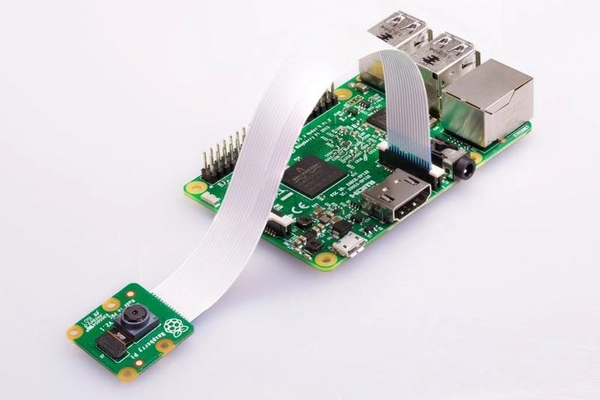
\includegraphics[scale=0.6]{"Grafiken/PiCam.png"}
	\caption{Raspberry Pi Camera Module an einen Raspi angeschlossen \footnote{Quelle: https://www.raspberrypi.org/products/camera-module-v2/}}
	\label{fig:picam}
\end{figure}
\footnotetext{Quelle: https://www.raspberrypi.org/products/camera-module-v2/}
\\
Bei unzureichenden Ergebnissen, sprich unscharfe Bilder aufgrund der Vibrationen der Drohne, hätten wir immer noch die Möglichkeit gehabt, eine andere Kamera zu verwenden. Da die PiCam keine optische Bildstabilisierung hat ist es noch ungewiss ob das Bild stabil genug für unsere Zwecke ist. Das zu Testen lag leider nicht mehr in unseren Möglichkeiten, da auf Grund der Covid-19 Situation keine weiteren Versuche  möglich waren.
\newpage
%0.5 Seite
\section{Aktorik}
Um zu wissen welche Aktorik man benötigt, haben wir zuerst eine Liste an Anforderungen erstellt, um zu wissen, was man mit der Aktorik überhaupt erreichen will. Die Aktorik geht außerdem sehr eng mit der Mechanik zusammen, weswegen wir in dem Bereich sehr nahe zusammen gearbeitet haben. Die Anforderungen waren wie folgt:
\begin{itemize}
	\item Greifen eines $10mm  \times 10mm \times 10mm$ großen Pakets
	\item Drohne in x-, y- und z- Richtung steuerbar
	\item sowohl Rotation um die z- Achse
\end{itemize}
Mit dieser Liste haben wir nun begonnen den Greifarm und die Drohne zu konzipieren, wobei das bei der Drohne eine deutlich einfachere Aufgabe war als bei dem Greifarm. Für die Drohne benutzen wir einen Mikrocontroller zur Regelung aller Flugbewegungen.
%1 Seite
\subsection{Hubzylinder}
Mit der aus Kapitel 3 bekannten Greifermechanik, stellte sich nun die Frage durch welche Art von Aktorik der Greifarm nun bewegt werden soll, auch hierzu haben wir wieder mehrere unterschiedliche Ideen gesammelt und miteinander verglichen. Bewertet haben wir nach folgenden Kriterien:
\begin{itemize}
	\item Komplexität
	\item Robustheit
	\item Gewicht
	\item Fehleranfälligkeit
	\item Effizienz
\end{itemize}
Zur Auswahl hatten wir schließlich einen Seilzug, angetrieben durch einen Elektromotor und einen Hubzylinder. Die meistgenutzten Hubzylinder sind entweder mit pneumatisch, hydraulisch oder elektrisch angetrieben, jedoch kommt für unsere Anwendung nur der elektrische Antrieb infrage, da Hydraulik und Pneumatik zu groß und schwer sind, denn dafür würde auch noch eine Pumpe benötigt werden.\\
\\
\newpage
\begin{figure}[h]
	\centering
	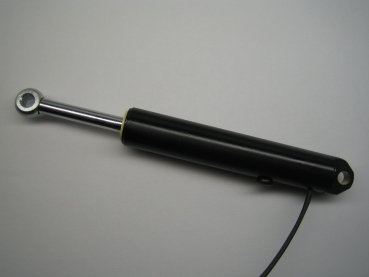
\includegraphics[scale=0.8]{"Grafiken/Hubzylinder.jpg"}
	\caption{Elektrischer Hubzylinder \footnote{Quelle: https://www.cti-modellbau.de/CTI-Hubzylinder/titan/}}
	\label{fig:hubzylinder}
\end{figure}
\footnotetext{Quelle: https://www.cti-modellbau.de/CTI-Hubzylinder/titan/}
Unsere Entscheidung ist zugunsten des elektrischen Hubzylinders gefallen, da dieser das beste Verhältnis zwischen Robustheit und Gewicht hat und dazu noch einen sehr simplen und robusten Aufbau hat. Der Hubzylinder, den wir in unserem Projekt verbaut haben, kommt aus dem Modellbau, da in diesem Segment Bauteile in der Größenordnung, wie wir sie benötigen oft vorkommen und genau für den Einsatzzweck an ferngesteuerten Modellen, was unsere Drohne im Grunde genommen auch ist.\\
Der Zylinder wird über einen Regler angesteuert, welcher die Endpositionen des Zylinders erkennen kann und bei einer Last von etwa 60N aufgrund des Überlastungsschutzes abschaltet.

%1.5 Seiten
\subsection{Flight-Controller}
Für die Steuerung der Drohne wird ein Controller benötigt, welchen wir über den Raspberry Pi ansteuern können. Hierfür haben wir den bereits am Institut vorhandenen Pixhawk Flight Controller benutzt. Dieser muss lediglich mit dem TX- und RX-Pin des Paspberry Pi verbunden werden. Außerdem empfiehlt es sich ebenfalls die Ground Verbindung des Raspberry Pis und die des Flight Controllers miteinander zu verbinden, da das die Signalqualität verbessert und es sonst zu Problemen kommen könnte.\\
\\
Nun stellt sich aber erstmal die Frage, warum wir überhaupt einen solchen Flight Controller benötigen und die Drohne nicht einfach direkt über den Raspberry Pi ansteuern. Das hat mehrere Gründe, zum einen ist die linux Version, welche sich auf dem Raspi befindet, nicht echtzeitfähig und somit kann es zu Problemen bei der Regelung kommen, wenn Beispielsweise der Raspi ausgelastet ist, würde die Regelung, welche der Quadrokopter benötigt, zu kurz kommen und somit der Flug sehr instabil werden. Zum anderen sparen wir uns damit sehr viel Zeit und Arbeitsaufwand, da der Flight Controller bereits die ganze Regelung für die Drohne besitzt und bereits mit unterschiedlichen Sensoren verbunden ist. Ein weiterer Vorteil dieser Methode ist, dass man die Drohne mit dem extra Flight Controller auch Manuel über eine Fernbedienung steuern kann, was bei einem Raspi nicht unmöglich ist, aber nochmal eine Menge mehr Aufwand bedeuten würde.
\begin{figure}[h]
	\centering
	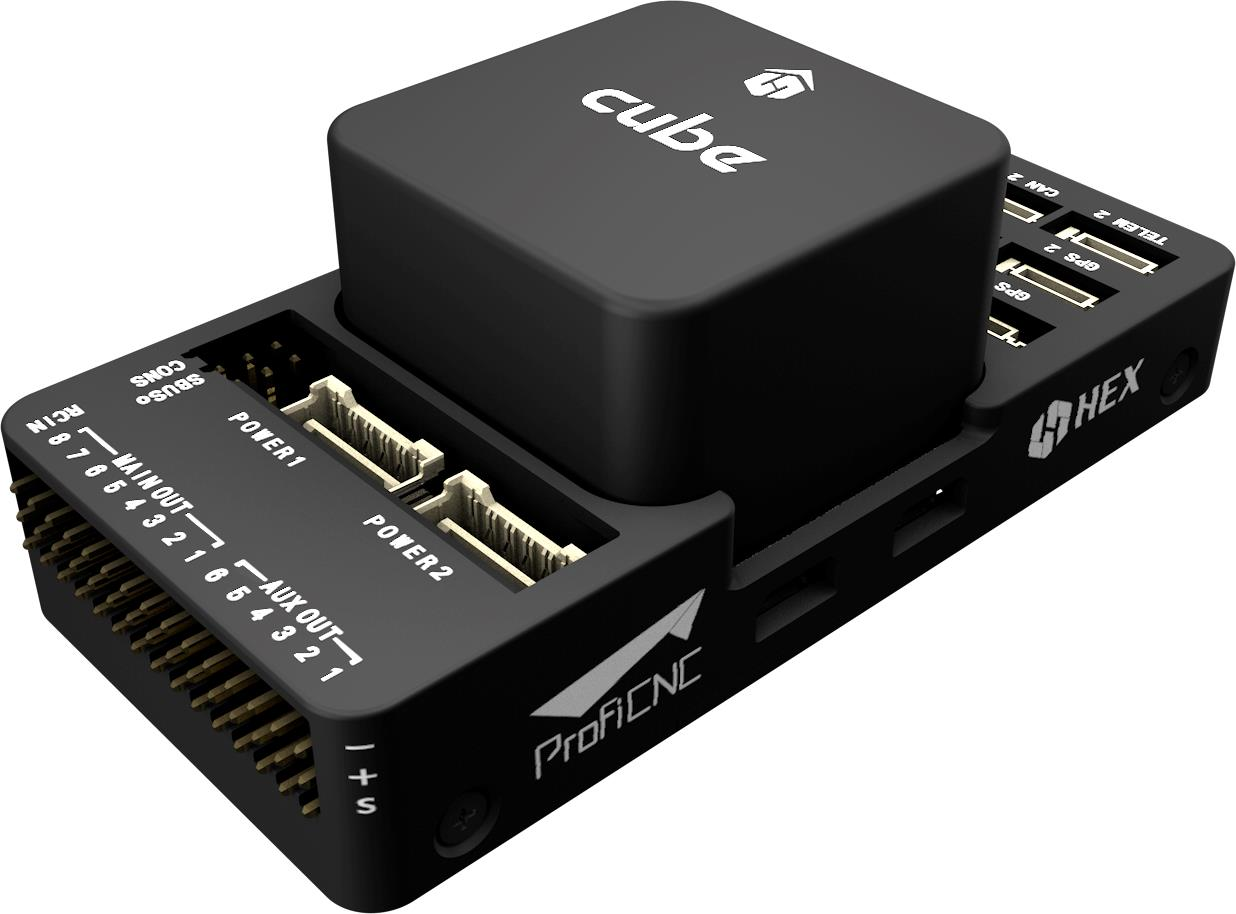
\includegraphics[scale=0.35]{"Grafiken/pixhawk2.png"}
	\caption{Flight Controller Pixhawk 2 \footnote{Quelle: https://docs.px4.io/v1.9.0/en/flight\_controller/pixhawk-2.html}}
	\label{fig:meine-grafik}
\end{figure}
\footnotetext{Quelle: https://docs.px4.io/v1.9.0/en/flight\_controller/pixhawk-2.html}
\\
\\
An diesem Controller sind nun die vier Elektromotore über ESCs (Electronic speed control) verbunden. Außerdem wird noch ein Empfänger für das Empfangen des Signales der Fernsteuerung angeschlossen, sowie bereits oben erwähnt das GPS Modul. Der Flight Controller bekommt später also nur noch Angaben wie zum Beispiel bewege dich zwei Meter nach oben und sorgt dann dafür, dass der Kopter sich auch genau zwei Meter nach oben bewegt. Das entlastet den Raspberry Pi extrem, sodass dieser genug Rechenleistung für die Bilderkennung übrig hat.

